\documentclass[a4j, 9pt]{ltjsarticle}

\usepackage{multicol}
\usepackage{amsmath, amssymb, amsfonts, mathtools} %数学系全般のパッケージ
\usepackage{tikz}
\usetikzlibrary{patterns}%斜線塗りを可能にする
\usepackage{mhchem} %化学用パッケージ
\usepackage{dotseqn}%式番号表示に詰まった点線を使えるようにする
\usepackage{cases}%場合分け内の各式に式番号を振れるようにする\begin{numcases}を追加する
\usepackage{pxrubrica} %ルビを振れるようにする\rubyを追加するパッケージ
\usepackage{boites} %breakboxを利用可能にする
\usetikzlibrary{calc}

%インデント追加に\spind を利用可能にする
\usepackage{xparse}
\newcommand{\splitindent}{\phantom{{}={}}}
\newcounter{CSplitIndent}
\NewDocumentCommand{\spind}{ O{1} }{
  \setcounter{CSplitIndent}{0}
  \whiledo{\value{CSplitIndent}<#1}{
    \splitindent
    \addtocounter{CSplitIndent}{1}
  }
}

%label属性のついたものの背景色を白で四角系で塗りつぶす
\tikzset{set label/.style={fill=white,rectangle,inner sep=1}}

%定義記号
\def\ldef{\coloneqq}
\def\define{\stackrel{\mathrm{def}}{=}}
\def\defineProposition{\stackrel{\mathrm{def}}{\Longleftrightarrow}}

%式番号表記の改善
\makeatletter
\@addtoreset{equation}{section}
\@addtoreset{figure}{section}
\@addtoreset{table}{section}
\renewcommand{\theequation}{%
  \ifnum\thesection>0
    \thesection.\arabic{equation}%
  \else
    \arabic{equation}%
  \fi
}
\renewcommand{\thefigure}{%
  \ifnum\thesection>0
    \thesection.\arabic{figure}%
  \else
    \arabic{figure}%
  \fi
}
\renewcommand{\thetable}{%
  \ifnum\thesection>0
    \thesection.\arabic{table}%
  \else
    \arabic{table}%
  \fi
}
\renewcommand{\appendix}{\par
  \setcounter{section}{0}%
  \setcounter{subsection}{0}%
  \gdef\presectionname{\appendixname}%
  \gdef\postsectionname{}%
  \gdef\thesection{\presectionname\@Alph\c@section\postsectionname}%
  \gdef\thesubsection{\@Alph\c@section.\@arabic\c@subsection}%
  %% 追加
  \renewcommand{\theequation}{\@Alph\c@section.\arabic{equation}}%
  \renewcommand{\thefigure}{\@Alph\c@section.\arabic{figure}}%
  \renewcommand{\thetable}{\@Alph\c@section.\arabic{table}}%
}
\makeatother

%ディスプレイスタイル
\def\ds{\displaystyle}

%文字の上にアクセント
\def\overdot#1{\overset{\text{\centerdot}}{#1}}

\setlength{\columnsep}{5mm}
\columnseprule=0.2mm

%multicols上でtableの代わりにfigurehere, tablehereを使う
\makeatletter
\newenvironment{tablehere}
  {\def\@captype{table}}
  {}
\newenvironment{figurehere}
  {\def\@captype{figure}}
  {}
\makeatother

\begin{document}

% 目次の出力
\tableofcontents
\clearpage

\part{基礎の確認}

  \section{集合論}
    数学でモデルを扱うとき集合論的に思考すると上手にそのモデルを扱うことができる。これは数学の問題を解く場合も同様である。では集合論とは何か、概要を確認しておこう。
    \begin{multicols}{2} %*を用いれば真ん中の直線を最初から最大にできる

      \subsection{集合の定義}
        集合とはその名の通り、いくつかのものをひとまとめにして考えた「ものの集まりのこと」である。
        特に集合論では「もの」のことを要素という。\par
        またある集合$\ds A$は他の集合$\ds B$と共通部分を持ったり、はたまたその集合$\ds A$自体が他の集合$\ds B$の一部分となるケースも考えられる。
        そのような場合順に「$\ds AとB$の共通部分」、「$\ds AはBの$部分集合」という。

        \begin{tikzpicture}[auto]
        
          %Ven diagram1
          \def \circleRadius{1}
          \def \leftCirclePoint{(0, 0)}
          \def \rightCirclePoint{(1, 0)}
          \def \centerPointOfShareArea{(0.5, 0)}
          \def \leftCircleNamePoint{(0, 1)}
          \def \rightCircleNamePoint{(1, 1)}

          %Ven diagram2
          \def \circleARadius{0.7}
          \def \circleBRadius{1}
          \def \circleAPoint{(4, -0.2)}
          \def \circleBPoint{(4, 0)}
          \def \circleANamePoint{(4, \circleARadius-0.2)}
          \def \circleBNamePoint{(4, \circleBRadius)}

          \scope
            %Aのベン図
            \clip \leftCirclePoint circle (\circleRadius);
            \fill [fill=white] \rightCirclePoint circle (\circleRadius);
          \endscope

          \scope
            %Bのベン図
            \clip \rightCirclePoint circle (\circleRadius);
            \fill [pattern=north west lines] \leftCirclePoint circle (\circleRadius);
          \endscope

          \draw \leftCirclePoint circle (\circleRadius);
          \draw \rightCirclePoint circle (\circleRadius);
          \node[set label, text=black] (A) at \leftCircleNamePoint {$\ds A$};
          \node[set label, text=black] (B) at \rightCircleNamePoint {$\ds B$};

          %共通部分ラベル
          \draw[semithick, -, stealth] \centerPointOfShareArea--(0.5, -1.5);
          \draw[semithick, -, stealth] (0.5, -1.5)--(-1, -1.5);
          \node[set label, text=black] (CAP) at (-1, -1.5) {$\ds AとBの共通部分$};


          \fill[pattern=north west lines] \circleAPoint circle (\circleARadius);
          \draw                           \circleAPoint circle (\circleARadius);
          \draw                           \circleBPoint circle (\circleBRadius);
          \node[set label, text=black] (A') at \circleANamePoint {$\ds A$};
          \node[set label, text=black] (B') at \circleBNamePoint {$\ds B$};

        \end{tikzpicture}

        \subsubsection{集合の例}
          例として「原子」という集合を考えてみよう。(ここでいう原子は化学の原子を指すものとする)\par
          原子には様々な種類があり、例えば水素原子\ce{_{1}H}や酸素原子\ce{_{8}O}などがある。
          このとき\ce{_{1}H}や\ce{_{8}O}は原子集合の要素であるといえる。\par
          またさらに水素元素\ce{H}や酸素元素\ce{O}はそれぞれ水素原子\ce{_{1}H}の全同位体を含んだ集合、酸素原子\ce{_{8}O}の全同位体を含んだ集合ゆえ原子集合の部分集合である。

      \subsection{集合論の記号}
        ここまでは言葉を用いて集合について少し語ってきた。しかしいちいち言葉で説明するのは少々面倒であり、しかも読みづらい。そこで記号を導入してみよう。

        \subsubsection{基本的な記法}
          例えば$\ds A$という集合を自然数$\ds 1 \thicksim 5$を要素に持つ集合として定義したい場合$\ds A \define \{ 1, 2, 3, 4, 5 \}$と書く。
          つまり要素を$\ds \{\}$で囲むことでそれらを要素に持つという意味を表すのである。
          この記法を\ruby{外延的記法}{がい|えん|てき|き|ほう}という。\par
          ついでこの場合$\ds 1$は$\ds A$の要素であるから、これを$\ds 1 \in A$と書く。\par
          
          %強制的に改段
          %\columnbreak
          
          また、同じ意味の定義で\par
          $\ds A \define \{ n \in \mathbb{N} \mid 1 \leq n \leq 5 \}$と表すこともできる。
          この場合は具体的に要素を書き出すことをせずに、\par
          $\ds \{ n \in ($母体となる集合$\ds ) \mid n$が満たす条件$\ds \}$といった具合に条件を満たすもので集合を定義する記法である。
          この記法は\ruby{内包的記法}{ない|ほう|てき|き|ほう}という。

          \paragraph{内包的記法の例}\mbox{}\\
            例えば次のように偶数全体の集合として$\ds A$を定義してみる。\par
            \begin{equation*}
              \begin{split}
                $\ds A \define \{ n \in \mathbb{Z} \mid \exists_{m \in \mathbb{Z}} [n = 2m] \}$\\
              \end{split}
            \end{equation*}
            このように存在記号や全称記号を用いた条件で定義されることはよくあるしとても簡潔でわかりやすい。

            \footnote{
              他の例として次のようなものがある\par
              開区間 $\ds (a, b) \define \{ x \in \mathbb{R} \mid a < x < b \}$,
              閉区間 $\ds [a, b] \define \{ x \in \mathbb{R} \mid a \leq x \leq b \}$
            }

        \vspace{9pt}\\
        
        以上の記号以外もまとめれば以下。

        %multicols上ではtableが使えないので代わりにtablehereを使う
        \begin{tablehere}
            \centering
            \begin{tabular}{ll}
                $\ds x \in X$                             & \cdots $\ds x$は$\ds X$の要素である\\
                $\ds x \notin X$                          & \cdots $\ds x$は$\ds X$の要素でない\\
                $\ds X \subset Y$                         & \cdots $\ds X$は$\ds Y$の部分集合である\\
                $\ds X \not\subset Y$                     & \cdots $\ds X$は$\ds Y$の部分集合でない\\
                $\ds X \cap Y$                            & \cdots $\ds X$と$\ds Y$の共通部分\\
                $\ds X \cup Y$                            & \cdots $\ds X$と$\ds Y$の和集合\\
                $\ds \varnothing$                         & \cdots 空集合\\
                $\ds | A |, \operatorname{Card}(A), n(A)$ & \cdots $\ds A$の要素数・濃度\\
                $\ds A = B$                               & \cdots $\ds A$と$\ds B$は同じ集合\\
                $\ds A \times B$                          & \cdots $\ds A$と$\ds B$の直積・デカルト積\\
                $\ds A^n$                                 & \cdots $\ds A$を自身で$\ds n$回直積をとったもの\\
            \end{tabular}
        \end{tablehere}

        \footnote{
          要素を持たない集合を空集合という。
        }

      \columnbreak

      \subsection{集合同士の積}
        実数に積という演算があるのと同じように集合間にも積の演算がある。それを直積、またはデカルト積という。ここではそれについてみておこう。\par

        \subsubsection{直積の定義}
          $\ds A,B \ne \varnothing$なる集合に対し、それらの要素$\ds a \in A, b \in B$を対にとった集合$\ds (a, b)$を直積と定義する。
          この対には「順序」があるため特に「順序対」という。
          式で定義すれば以下。\par
          $\ds A \times B \define \{ (a, b) \mid a \in A, b \in B \}$\par
          直積は「それぞれの要素を対にとった集合」として定義されているので、この演算には一般に交換法則が成立しないことがわかる。

          \footnote{
            直積をとる集合の片方または両者が空集合の場合順序対の作りようがないためその結果は空集合として定義されている。\par
            $\ds A = \varnothing \vee B = \varnothing$のとき$\ds A \times B \define \varnothing$
          }
          
          \paragraph{交換法則が成立しない一つの例}
            \begin{equation*}
              \begin{split}
                $\ds A \define \{ a, b, c \}, B \define \{ 1, 2 \}$\\
              \end{split}
            \end{equation*}
            とする。$\ds A$と$\ds B$の直積$\ds A \times B$を計算してみよう。\par
            例えば$\ds a \in A, 1 \in B$であるから求めるべき直積には積の順と同順の順序対$\ds (a, 1)$が要素として存在する。\par
            では逆に$\ds B \times A$の場合は$\ds (1, a)$が要素として存在する。しかしこの場合$\ds (a, 1)$は要素として存在しない。
            順序対は対の順序を考慮するから$\ds (a, 1) \ne (1, a)$である。\par
            ゆえに$\ds A \times B = B \times A$はこの場合成り立たない。\par

          \vspace{9pt}\\

          以上のように一般に直積は$\ds A \times B \ne B \times A$である。\par
          しかし、特例としてこれが成立する場合もある。その例は次のような場合である。

          \paragraph{交換法則が成立する特例}

            \begin{equation*}
              \begin{split}
                $\ds A, B \define \{ 1, 2\}$\\
              \end{split}
            \end{equation*}

            とする。ここで$\ds A \times B$を考えてみると

            \begin{equation*}
              \begin{split}
                $\ds 1 \in A, 1 \in B$\\
              \end{split}
            \end{equation*}

            であるから考えている直積には順序対$\ds (1, 1)$が要素として存在する。\par
            実際にすべて書き出して計算すると\par

            \begin{equation*}
              \begin{split}
                $\ds A \times B = \{ (1, 1), (1, 2), (2, 1), (2, 2) \}$\\
              \end{split}
            \end{equation*}

            となっている。もしこれをひっくり返したとしても結果は同じである。\par
            よってこの場合$\ds A \times B = B \times A$が成立する。\par

          \vspace{9pt}\\

          この場合なぜ交換法則が成立するのか考えてみると、直積をとった集合同士が全く同じ要素を持つ集合同士であったことが要因であることがわかる。\par
          (また、自身で直積をとった場合$\ds A \times A = A^2$と表し、一般に$\ds n$回直積をとった時$\ds A^n$と表す。)\par
          ゆえにこれを一般化すると次のように言える。(ただし有限集合の場合に限る)\par

          \begin{eqnarray}
            \begin{split}
              $\ds ( A = \varnothing \vee B = \varnothing \vee A = B ) \Longleftrightarrow $&$\ds A \times B = B \times A$ \label{eq:ex-cartesian-product}
            \end{split}
          \end{eqnarray}

          これは対偶をとってもわかる通り直積に持っていてほしい特性が論理的に正しく保持されていることも確認できる。\par

          \begin{equation*}
            \begin{split}
              \eqref{eq:ex-cartesian-product}
              $\ds \Longleftrightarrow ( A \times B \ne B \times A \Longleftrightarrow ( A \ne \varnothing \wedge B \ne \varnothing \wedge A \ne B ) )$\\
            \end{split}
          \end{equation*}

        \subsubsection{直積の要素の個数(濃度)}
          直積の要素の個数はどのように求まるか、先ほどの積の交換法則が成立しない例の状況で考えてみよう。\par
          このとき$\ds A \times B$を計算してみると

          \begin{equation*}
            \begin{split}
              $\ds A \times B = \{ (a, 1), (a, 2), (b, 1), (b, 2), (c, 1), (c, 2) \}$\\
            \end{split}
          \end{equation*}

          直積の要素は「順序対」であったからこの場合の要素数は$\ds 6$である。\par
          これを一般の集合(有限集合のとき)の場合にも適用できるように考えてみよう。次のように表にしてみるとわかりやすいだろう。

          \vspace{9pt}\\

          \begin{tablehere}
            \centering
            \label{tab:hogehoge}
            \begin{tabular}{c|ccc}
                    & $\ds a$       & $\ds b$       & $\ds c$     \\ \hline
                1   & $\ds (a, 1)$  & $\ds (b, 1)$  & $\ds (c, 1)$\\
                2   & $\ds (a, 2)$  & $\ds (b, 2)$  & $\ds (c, 2)$\\
            \end{tabular}
          \end{tablehere}

          \vspace{9pt}\\

          つまり要素数はこの表で順序対が作る長方形の面積のようなものと対応していることがわかる。\par
          よって一般に
          
          \begin{equation*}
            \begin{split}
              $\ds | A \times B | = | A | \times | B |$\\
            \end{split}
          \end{equation*}

          と表せることがわかる。(ただし有限集合同士の直積の場合のみ)

      \columnbreak

      \subsection{実数平面や実数空間の表現}
        実数全体の集合$\ds \mathbb{R}$は他の視点から見ると実数の数直線を表す集合と考えられる。\par
        では実数平面や実数空間などは集合を使ってどのように表せるだろうか。
        ここで次のような直積を考えてみる。

        \begin{equation*}
          \begin{split}
            $\ds \mathbb{R} \times \mathbb{R} = \mathbb{R}^2$
          \end{split}
        \end{equation*}

        これは幾何的に解釈すると、実数の数直線同士を平行でない向きに並べたときにできる平面のすべての点を要素に持つ集合である。
        それはまさに実数平面のことである。

        \begin{tikzpicture}

          \coordinate[label=below  left:O] (O) at (0,0); %原点O
          \coordinate (XS) at (-1,0); %x軸最小
          \coordinate (XL) at (1,0); %x軸最大
          \coordinate (YS) at (0,-1); %y軸最小
          \coordinate (YL) at (0,1); %y軸最大
          \draw[semithick,->,>=stealth] (XS)--(XL) node[right] {$\mathbb{R}$}; %x軸
          \draw[semithick,->,>=stealth] (YS)--(YL) node[above] {$\mathbb{R}$}; %y軸

        \end{tikzpicture}
        
        このことを意識して直積を書き直すと

        \begin{equation*}
          \begin{split}
            $\ds \mathbb{R}^2 = \{ (x, y) \mid x \in \mathbb{R}, y \in \mathbb{R} \}$
          \end{split}
        \end{equation*}

        と書ける。\par

        \vspace{9pt}\\

        同様の議論で実数空間($\ds 3$次元空間)も次のような直積で表せる。

        \begin{equation*}
          \begin{split}
            $\ds \mathbb{R}^3 = \{ (x, y, z) \mid x \in \mathbb{R}, y \in \mathbb{R}, z \in \mathbb{R} \}$
          \end{split}
        \end{equation*}

        \begin{figurehere}
          \centering
          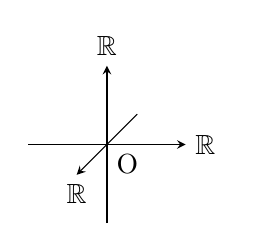
\begin{tikzpicture}

            \draw[-stealth](-1,0,0) -- (1,0,0) node[right]{$\mathbb{R}$};
            
            \draw[-stealth](0,-1,0) -- (0,1,0) node[above]{$\mathbb{R}$};
            
            \draw[-stealth](0,0,-1) -- (0,0,1) node[below]{$\mathbb{R}$};
            
            \draw (0,0,0) node[below right]{O};
          
          \end{tikzpicture}
        \end{figurehere}

        これを用いれば直積の交換法則が不成立な理由も次のように考えて直観的に理解できる。\par

        \subsubsection{幾何的に直積の交換法則が不成立であることを確認してみる}
          ある点$\ds (a, b)$を考えてみよう。(ただし$\ds a \ne b$とする。)\par
          二次元平面上では$\ds a \ne b$ならば$\ds (a, b) \ne (b, a)$である。\par
          これは順序対が反転すると幾何的に異なる量へ変化するためである。

          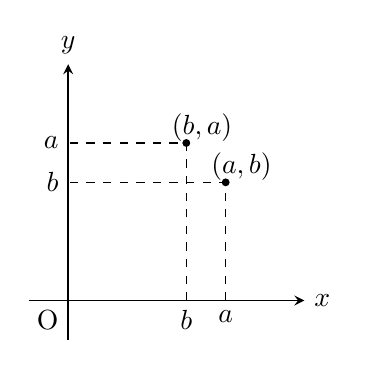
\begin{tikzpicture}
          
            \coordinate[label=below  left:O] (O) at (0,0); %原点O
            \coordinate (XS) at (-0.5,0); %x軸最小
            \coordinate (XL) at (3,0); %x軸最大
            \coordinate (YS) at (0,-0.5); %y軸最小
            \coordinate (YL) at (0,3); %y軸最大
            \draw[semithick,->,>=stealth] (XS)--(XL) node[right] {$x$}; %x軸
            \draw[semithick,->,>=stealth] (YS)--(YL) node[above] {$y$}; %y軸
            
            % (a, b)
            \coordinate (P1) at (2,1.5); %右頂点
            \fill (P1) circle (0.05); %点の塗りつぶし
            \node (x) at (2.2, 1.7) {$\ds (a, b)$};%座標の可視化
            
            % (b, a)
            \coordinate (P2) at (1.5,2); %右頂点
            \fill (P2) circle (0.05); %点の塗りつぶし
            \node (x) at (1.7, 2.2) {$\ds (b, a)$};%座標の可視化
            
            \draw[dashed] ($(XS)!(P1)!(XL)$)node[below]{$\ds a$}--(P1)--($(YS)!(P1)!(YL)$)node[left]{$\ds b$};
            \draw[dashed] ($(XS)!(P2)!(XL)$)node[below]{$\ds b$}--(P2)--($(YS)!(P2)!(YL)$)node[left]{$\ds a$};
              %右頂点から各軸への垂線

          \end{tikzpicture}

          すなわちこれは幾何的に順序対が異なるものであることを説明しており、直積の順序で順序対が変化することが異なる量へ変化していることの根拠である。\par
          実際このことは直積(特に順序対)の定義であった。
          それに対しこの幾何的説明は、順序対が対の順序を考慮することの合理性を示していると考えられる。

        \subsection{参考: ユークリッド空間}
          先ほど$\ds \mathbb{R}$の直積を積み立てることで$\ds 2, 3$次元空間を集合で表現することができた。
          ではここでこれの一般化をしてみよう。\par
          次のように$\ds N \in \mathbb{N}$個の直積を考えてみる。

          \begin{equation*}
            \begin{split}
              $\ds \mathbb{R}^N = \{ (x_1, x_2, \cdots , x_N) \mid x_1 \in \mathbb{R}, x_2 \in \mathbb{R}, \cdots , x_N \in \mathbb{R} \}$
            \end{split}
          \end{equation*}

          % \[
          %   \left(
          %     \begin{tabular}{l}
          %       または次のようにも表せる。\\
          %       \begin{equation*}
          %         \begin{split}
          %           $\ds \mathbb{R}^3 = \{ (x, y, z) \mid x \in \mathbb{R}, y \in \mathbb{R}, z \in \mathbb{R} \}$\\
          %         \end{split}
          %       \end{equation*}
          %     \end{tabular}
          %   \right)
          % \]
          
          ここに得られた集合$\ds \mathbb{R}^N$をユークリッド空間という。\par
          つまり任意の$\ds N \in \mathbb{N}$に対して呼ぶので$\ds \mathbb{R}^2$の$\ds 2$次元平面や$\ds \mathbb{R}^3$の$\ds 3$次元空間もユークリッド空間である。
      
      \subsection{実数集合の最大値・最小値}
        実数空間$\ds \mathbb{R}$上には「大小関係 $\ds \leq$」と呼ばれる二項関係が定義されており、これは全順序としての性質

        \begin{numcases}
          $\ds \forall_{x \in \mathbb{R}} [ x \leq x]$ & \label{ax:inequality-to-real-1} \\
          $\ds \forall_{x, y \in \mathbb{R}} [ (x \leq y \wedge y \leq x) \Rightarrow x = y ]$ & \label{ax:inequality-to-real-2} \\
          $\ds \forall_{x, y, z \in \mathbb{R}} [ (x \leq y \wedge y \leq z) \Rightarrow x \leq z ]$ & \label{ax:inequality-to-real-3} \\
          $\ds \forall_{x, y \in \mathbb{R}} [ x \leq y \vee y \leq x ]$ & \label{ax:inequality-to-real-4}
        \end{numcases}

        を満たすことを公理として認める。\par
        
        \subsubsection{各公理の具体例}
          \paragraph{\eqref{ax:inequality-to-real-1}} $\ds 0.999\cdots \leq 1$
          \paragraph{\eqref{ax:inequality-to-real-2}} はさみうちの定理
          \paragraph{\eqref{ax:inequality-to-real-3}} $\ds (1 \leq 1.1 \wedge 1.1 \leq 1.2) \Rightarrow 1 \leq 1.2$
          \paragraph{\eqref{ax:inequality-to-real-4}} これは具体例よりも主張内容を説明したほうがわかりやすい。\par
            任意の$\ds x, y \in \mathbb{R}$には必ず$\ds x \leq y$または$\ds y \leq x$が成立する。仮に$\ds x = y$であった場合も\eqref{ax:inequality-to-real-1}より成立する。\par

        この下で、次のものを定義する。

        \begin{breakbox}
          任意の$\ds x, y \in \mathbb{R}$に対し、
          \begin{equation*}
            \begin{split}
              $\ds x < y \defineProposition (x \leq y \land x \ne y)$
            \end{split}
          \end{equation*}
        \end{breakbox}

        また、実数空間$\ds \mathbb{R}$の空でない部分集合$\ds A$があるとき、ある$\ds a \in A$が任意の$\ds x \in A$以上であるとき、この$\ds a$を$\ds A$の最大値(最大元)とよぶ。\par
        つまり

        \begin{breakbox}
          \begin{equation*}
            \begin{split}
              $\ds \max A = a \defineProposition \exists_{a \in A} [ \forall_{x \in A} [ x \leq a ] ]$
            \end{split}
          \end{equation*}
        \end{breakbox}

        \footnote{
          定義に「以下 $\ds \leq$」を用いる理由は、任意の$\ds x \in A$としているため$\ds x = a$の場合もあるので、それを考慮しているためである。
        }

        次に、同様の状況$\ds A \subset \mathbb{R} \land A \ne \varnothing$において、ある$\ds a \in A$が任意の$\ds x \in A$以下であるとき、この$\ds a$を$\ds A$の最小値(最小元)とよぶ。\par
        つまり

        \begin{breakbox}
          \begin{equation*}
            \begin{split}
              $\ds \min A = a \defineProposition \exists_{a \in A} [ \forall_{x \in A} [ a \leq x ] ]$
            \end{split}
          \end{equation*}
        \end{breakbox}

        \footnote{
          今紹介したもの以外の話や詳しい議論は以下を参照\par
          https://wiis.info/math/real-number/definition-of-real-number/magnitude-relation/\par
          https://wiis.info/math/real-number/definition-of-real-number/maximu-value-and-minimum-value/
        }

    \end{multicols}

  \newpage

  \section{写像}
    前節では集合論の概要を説明した。ついでここでは集合間を関係づける概念、写像についてみておこう。
    \begin{multicols}{2}

      \subsection{写像の定義}
        $\ds X, Y$を空でない集合とする。\par
        任意の$\ds x \in X$に対し、ある$\ds y \in Y$が一意に定まるとき、このような対応規則を「$\ds X$から$\ds Y$への写像」と呼ぶ。\par
        また$\ds X, Y$が数を要素とする集合の場合特に関数と呼ぶ。つまり$\ds 関数 \subset 写像$である。\par
        簡潔に表現すれば以下。

        \vspace{9pt}\\

        $\ds f:X \mapsto Y \defineProposition \forall_{x \in X} [\exists!_{y \in Y} [y = f(x)]]$

        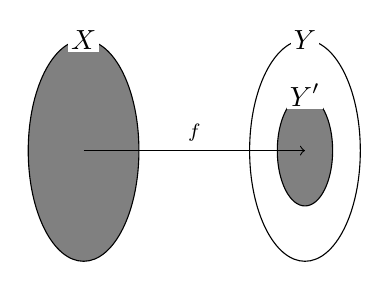
\begin{tikzpicture}[auto]
        
          %Xのベン図
          \fill[color=black!50!white, draw=black] (0,0) ellipse (20pt and 40pt);
          \node[set label,text=black] (X) at (0, 40pt) {$\ds X$};

          %Yのベン図
          \draw (80pt,0) ellipse (20pt and 40pt);
          \fill[color=black!50!white, draw=black] (80pt, 0) ellipse (10pt and 20pt); % black!50!white で黒と白50%
          \node[set label,text=black] (Y) at (80pt, 40pt) {$\ds Y$};
          \node[set label,text=black] (Y') at (80pt, 20pt) {$\ds Y'$};

          %写像f
          \draw[->] (0, 0) to node {$\scriptstyle f$} (80pt, 0);

        \end{tikzpicture}

      \subsection{定義域・値域}
        $\ds f:X \mapsto Y$において\par
        \begin{cases}
          $\ds X$を$\ds f$の定義域\\
          $\ds Y'(\subset Y)$を$\ds f$の値域\\
        \end{cases}
        という。\par

        値域$\ds R_f$の具体的な定義は以下。
      
        \vspace{9pt}\\

        $\ds R_f \defineProposition \{y \in Y \mid \exists_x [x \in X \wedge y=f(x)]\}$

        % \footnote{
        %   $\ds \exists_x [x \in X \wedge y=f(x)]$は自由変項$\ds y$が残るため$\ds y$の条件と言える。
        % }

      \subsection{単射(行先がかぶらない写像)}
        写像にはいくつか特性が存在する。その特性の一つを有する写像が単射と呼ばれるものである。\par
        $\ds f:X \mapsto Y$が単射であるとは、任意の$x,x'\in X$に対して「$\ds x \ne x' \Longrightarrow f(x) \ne f(x')$」が成立することである。\par
        つまり簡潔に表せば以下。

        \begin{equation*}
          \begin{split}\notag
            $\ds f:X \mapsto Yが単射$     & $\defineProposition      \forall_{x,x'\in X} [x \ne x' \Longrightarrow f(x) \ne f(x')]$\\
                                          & $\ds \Longleftrightarrow  \forall_{x,x'\in X} [f(x) = f(x') \Longrightarrow x = x']$\\
          \end{split}
        \end{equation*}

        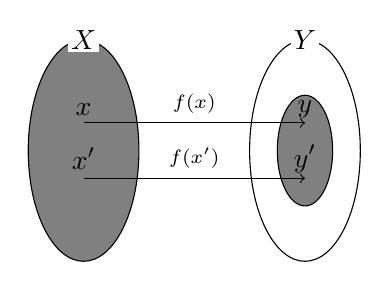
\begin{tikzpicture}[auto]
        
          %Xのベン図
          \fill[color=black!50!white, draw=black] (0,0) ellipse (20pt and 40pt);
          \node[set label, text=black] (X) at (0, 40pt) {$\ds X$};

          %Yのベン図
          \draw (80pt,0) ellipse (20pt and 40pt);
          \fill[color=black!50!white, draw=black] (80pt, 0) ellipse (10pt and 20pt); % black!50!white で黒と白50%
          \node[set label, text=black] (Y) at (80pt, 40pt) {$\ds Y$};

          %x->y
          \node (x) at (0, 15pt) {$\ds x$};
          \node (y) at (80pt, 15pt) {$\ds y$};
          \draw[->] (0, 10pt) to node {$\scriptstyle f(x)$} (80pt, 10pt);

          %x'->y'
          \node (x') at (0, -3pt) {$\ds x'$};
          \node (y') at (80pt, -3pt) {$\ds y'$};
          \draw[->] (0, -10pt) to node {$\scriptstyle f(x')$} (80pt, -10pt);

        \end{tikzpicture}

      \subsection{全射}
        写像の特使の一つを有するものを単射と言った。他にも全射と呼ばれるものもある。\par
        $\ds f:X \mapsto Y$が全射であるとは、任意の$y \in Y$に対して、ある$\ds x \in X$が存在し$\ds f(x)=y$となることである。\par
        つまり簡潔に表せば以下。

        \begin{equation*}
          \begin{split}\notag
            $\ds f:X \mapsto Yが全射$     & $\defineProposition      \forall_{y\in Y} [\exists_{x\in X} [f(x) = y]]$\\
          \end{split}
        \end{equation*}

        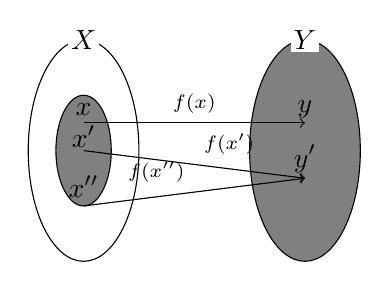
\begin{tikzpicture}[auto]
        
          %Xのベン図
          \draw (0,0) ellipse (20pt and 40pt);
          \fill[color=black!50!white, draw=black] (0, 0) ellipse (10pt and 20pt); % black!50!white で黒と白50%
          \node[set label, text=black] (X) at (0, 40pt) {$\ds X$};

          %Yのベン図
          \fill[color=black!50!white, draw=black] (80pt,0) ellipse (20pt and 40pt);
          \node[set label, text=black] (Y) at (80pt, 40pt) {$\ds Y$};

          %x->y
          \node (x) at (0, 15pt) {$\ds x$};
          \node (y) at (80pt, 15pt) {$\ds y$};

          %x'->y'
          \node (x') at (0, 5pt) {$\ds x'$};
          \node (y') at (80pt, -3pt) {$\ds y'$};

          %x''->y'
          \node (x'') at (0, -13pt) {$\ds x''$};

          \draw[->] (0, 10pt) to node {$\scriptstyle f(x)$} (80pt, 10pt);
          \draw[->] (0, 0) to node {$\scriptstyle f(x')$} (80pt, -10pt);
          \draw[->] (0, -20pt) to node {$\scriptstyle f(x'')$} (80pt, -10pt);

        \end{tikzpicture}

        \subsection{全単射(1対1対応、変換)}
        既に写像の特性を持つものを2つ紹介したが、これらの特性を同時に有するものも存在する。それを全単射といい、単射と全射それぞれの定義から成る合成命題で定義される。\par
        $\ds f:X \mapsto Y$が全単射であるとは、$\ds f$が単射かつ全射であるときをいう。\par
        また、定義域と値域が等しいことよりこの対応を1対1対応とも呼び、さらに互いの集合間をすべての要素が行き来できることより変換とも呼ぶ。(ただし変換に関しては必ずしも1対1対応でなくてもよい。)\par
        つまり簡潔に表せば以下。

        \begin{multline*}
          $\ds f:X \mapsto Yが全単射 \defineProposition \forall_{x,x'\in X} [f(x) = f(x') \Longrightarrow x = x']$\\
                                                        $\ds \wedge \forall_{y\in Y} [\exists_{x\in X} [f(x) = y]]$
        \end{multline*}

        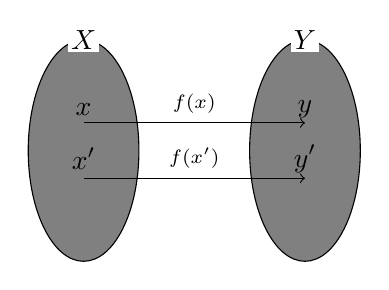
\begin{tikzpicture}[auto]
        
          %Xのベン図
          \fill[color=black!50!white, draw=black] (0,0) ellipse (20pt and 40pt);
          \node[set label, text=black] (X) at (0, 40pt) {$\ds X$};

          %Yのベン図
          \fill[color=black!50!white, draw=black] (80pt,0) ellipse (20pt and 40pt);
          \node[set label, text=black] (Y) at (80pt, 40pt) {$\ds Y$};

          %x->y
          \node (x) at (0, 15pt) {$\ds x$};
          \node (y) at (80pt, 15pt) {$\ds y$};
          \draw[->] (0, 10pt) to node {$\scriptstyle f(x)$} (80pt, 10pt);

          %x'->y'
          \node (x') at (0, -3pt) {$\ds x'$};
          \node (y') at (80pt, -3pt) {$\ds y'$};
          \draw[->] (0, -10pt) to node {$\scriptstyle f(x')$} (80pt, -10pt);

        \end{tikzpicture}

    \end{multicols}

  \section{対称式}
    対称式とは変数を入れ替えても形が変わらない多項式のことである。まず多項式がどんなものか確認して、次に対称式の性質や対称式の基本定理について議論しよう。  

    \begin{multicols*}{2}
      
      \subsection{多項式・整式の定義}
        多項式(整式)とは「数」と「変数」を和と積によって作られる
          (線形結合\footnote{
            線形結合の具体的な定義は
            「体$\ds \mathbb{F}$上の線形空間\boldsymbol{V}に対する$\ds \boldsymbol{v_1}, \boldsymbol{v_2}, \cdots , \boldsymbol{v_n} \in \boldsymbol{V}$の線形結合とは
            $\ds c_1 \boldsymbol{v_1} + c_2 \boldsymbol{v_2} + \cdots + c_n \boldsymbol{v_n} (c_1, c_2, \cdots , c_n \in \mathbb{F})$で表されるベクトルのこと」
          }と言ったりする)
        式のことである。\par
        たとえば$\ds 3x^3 + 5x^2 - x + 10$は$\ds x$を変数とする多項式である。
        また、多項式は変数を複数持つ場合も言う。\par
        変数が$\ds 1$つの場合の多項式の一般形を書くと

        \begin{equation*}
          \begin{split}
            $\ds a_n x^n + a_{n-1} x^{n-1} + \cdots + a_1 x + a_0 ( = \sum_{k=0}^n a_k x^k )$\\
          \end{split}
        \end{equation*}

        ここに各々の$\ds x_k$において$\ds a_k x^k$のようにして積で結ばれる。この積で結ばれた塊を項と呼び、$\ds a_k$を$\ds x^k$の係数と呼ぶ。
        特に$\ds 0$次の項を定数項と呼ぶ。\par
        また、一般には和を持たない多項式(例えば$\ds 4x^2$など)も存在し、それらを単項式と呼ぶ。\par
        ゆえに$\ds 単項式 \subset 多項式 = 整式$である。

        \subsubsection{多項式・整式でないもの}
          紛らわしいものに次のようなものがある。

          \begin{equation*}
            \begin{split}
              &・$\ds \frac{1}{x} = x^{-1}$\\
              &・$\ds x^\frac{1}{2} = \sqrt{x}$\\
              &・$\ds \sum_{n=0}^\infty x^n = 1 + x + x^2 + \cdots$\\
            \end{split}
          \end{equation*}

          これらはすべて多項式・整式ではない。(ゆえに単項式でもない)\par
          これらはx上から順に「有利式・分数式」、(名前なし)、「級数」という。
      
      \columnbreak

      \subsection{対称式の定義}
        先に述べたように対称式とは変数を入れ替えても変わらない多項式のことである。
        例えば次のような$\ds 2$変数の多項式のようなものをいう。

        % \begin{equation}
        \begin{equation*}
          \begin{split}
            % $\ds f(x, y) \ldef x^2 + xy + y^2$ \label{sym_1}\\
            $\ds f(x, y) \ldef x^2 + xy + y^2$\\
          \end{split}
        % \end{equation}
        \end{equation*}

        この式で$\ds x, y$を入れ替えてみても次の通り

        % \begin{equation}
        \begin{equation*}
          \begin{split}
            % $\ds f(y, x) = y^2 + yx + x^2$ \label{sym_2}\\
            $\ds f(y, x) $  &$\ds = y^2 + yx + x^2$\\
                            &$\ds = f(x, y)$\\
          \end{split}
        % \end{equation}
        \end{equation*}

        % \eqref{sym_1}と\eqref{sym_2}は全く同じ多項式である。
        これらは全く同じ多項式である。\par
        今見たものは$\ds 2$変数のものであったが、さらには例として次のような$\ds n$変数の対称式を考えられる。

        \begin{equation*}
          \begin{split}
            $\ds f(x_1, x_2, \cdots , x_n) \ldef \sum_{k=1}^n x_k^7$\\
          \end{split}
        \end{equation*}

        これも任意の$\ds x_k (1 \leq k \leq n)$を任意の分だけ入れ変えてもすべての場合で同じ多項式となる。\par
        例えば$\ds x_2$と$\ds x_n$を入れ替えてみても

        \begin{equation*}
          \begin{split}
            $\ds f(x_1, x_n, \cdots , x_2) $  & $\ds = x_1^7 + x_n^7 + \sum_{k=3}^{n-1} x_k^7 + x_2^7$\\
                                              & $\ds = x_1^7 + x_2^7 + \sum_{k=3}^{n-1} x_k^7 + x_n^7$\\
                                              & $\ds = \sum_{k=1}^{n} x_k^7$\\
                                              & $\ds = f(x_1, x_2, \cdots , x_n)$
          \end{split}
        \end{equation*}

        のように成立する。

      \columnbreak

      \subsection{基本対称式の定義}
        基本対称式とは$\ds n$個の変数$\ds x_1, x_2, \cdots , x_n$らを要素にもつ集合$\ds X$、つまり$\ds X \ldef \{ x_k \mid k \in \mathbb{N} \wedge 1 \leq k \leq n \}$なる集合$\ds X$から
        $\ds 1 \leq k \leq n$を満たす異なる$\ds k$個の変数を掛け合わせたものをすべての場合で作り、それらの和をとってできる対称式のことをいう。
        この基本対称式は後に議論する「対称式の基本定理」に登場し、対称式に関してとても重要な役割を果たすため天から降ってきたようなやり方だがここでとりあえず定義しておく。\par
        この$\ds k$個の変数の場合の基本対称式を$\ds \sigma_k(x_1, x_2, \cdots , x_n)$とすると以下すべてが該当する。

        \begin{equation*}
          \begin{cases}
            &\begin{split}
              $\ds \sigma_1(x_1, x_2, \cdots , x_n)$ & $\ds = x_1 + x_2 + \cdots + x_n$\\
              &$\ds = \sum_{k=1}^n x_k$
            \end{split}\\
            &\begin{split}
                $\ds \sigma_2(x_1, x_2, \cdots , x_n)$ & $\ds = x_1 x_2 + x_1 x_3 + $\\
              & \quad \cdots $\ds + x_1 x_n + x_2 x_3 + x_2 x_4 +$\\
              & \quad \quad \cdots $\ds + x_{n-1} x_n$\\
              & $\ds = \sum_{k_1=1}^{n-1} \sum_{k_2=2}^{n} x_{k_1} x_{k_2}$
            \end{split}\\
            &\begin{split}
              $\ds \sigma_3(x_1, x_2, \cdots , x_n)$ & $\ds = x_1 x_2 x_3 + x_1 x_2 x_4 + $\\
              & \quad \cdots $\ds + x_{n-2} x_{n-1} x_n$\\
              & $\ds = \sum_{k_1=1}^{n-2} \sum_{k_2=2}^{n-1} \sum_{k_3=3}^{n} x_{k_1} x_{k_2} x_{k_3}$\\
              & $\ds = \sum_{k_1=1}^{n-2} \sum_{k_2=2}^{n-1} \sum_{k_3=3}^{n} \prod_{m=1}^3 x_{k_m}$
            \end{split}\\
            & \vdots \\
            &\begin{split}
              $\ds \sigma_l(x_1, x_2, \cdots , x_n)$ & $\ds = \sum_{k_1=1}^{n-l+1} \cdots \sum_{k_{l-1}=l-1}^{n-1} \sum_{k_l=l}^n \prod_{m=1}^l x_{k_m}$
            \end{split}\\
            & \vdots \\
            &\begin{split}
              $\ds \sigma_n(x_1, x_2, \cdots , x_n)$ & $\ds = x_1 x_2 x_3 \cdots x_n$\\
              & $\ds = \prod_{k=1}^n x_k$
            \end{split}\\
          \end{cases}
        \end{equation*}

        \subsubsection{基本対称式の具体例}
          これだけ見てもピンとこないだろうから簡単に$\ds n=2, 3$の場合を見てみよう。

          \paragraph{具体例$\ds 1$}\mbox{}\\
            $\ds n=2$の場合対称式の説明をしたときと照らせ合わせるように$\ds x_1 = x, x_2 = y$とすると

            \begin{equation*}
              \begin{cases}
                &$\ds \sigma_1(x, y) = x + y$\\
                &$\ds \sigma_2(x, y) = xy$\\
              \end{cases}
            \end{equation*}

            確かにこれらは対称式である。

            \subparagraph{類似: $\ds 2$次方程式の解と係数の関係}

              \begin{equation*}
                \begin{split}
                  $\ds 2$次方程式$\ds ax^2 + bx + c = 0 (\Longleftrightarrow x^2 + \frac{b}{a}x + \frac{c}{a} = 0)$\\
                \end{split}
              \end{equation*}
              
              の$\ds 2$解を$\ds x= \alpha, \beta$としたとき、解と係数の関係として

              \begin{equation*}
                \begin{split}
                  $\ds \alpha + \beta = - \frac{b}{a} \wedge \alpha \beta = \frac{c}{a} \Longleftrightarrow x^2 + \frac{b}{a}x + \frac{c}{a} = 0$\\
                \end{split}
              \end{equation*}

              が成立する。

          \paragraph{具体例$\ds 2$}\mbox{}\\
            次に$\ds n=3$の場合も同様に$\ds x_1 = x, x_2 = y, x_3 = z$として

            \begin{equation*}
              \begin{cases}
                &$\ds \sigma_1(x, y, z) = x + y + z$\\
                &$\ds \sigma_2(x, y, z) = xy + yz + zx$\\
                &$\ds \sigma_3(x, y, z) = xyz$\\
              \end{cases}
            \end{equation*}

            これも対称式であることが確認できた。

            \subparagraph{類似: $\ds 3$次方程式の解と係数の関係}

              \begin{equation*}
                \begin{split}
                  $\ds 3$次方程式$\ds ax^3 + bx^2 + cx + d = 0 (\Longleftrightarrow x^3 + \frac{b}{a}x^2 + \frac{c}{a}x + \frac{d}{a} = 0)$\\
                \end{split}
              \end{equation*}

              の$\ds 3$解を$\ds x= \alpha, \beta, \gamma$としたとき、解と係数の関係として

              \begin{equation*}
                \begin{split}
                  &$\ds \alpha + \beta + \gamma = - \frac{b}{a} \wedge \alpha \beta + \beta \gamma + \gamma \alpha = \frac{c}{a} \wedge \alpha \beta \gamma = \frac{d}{a}$\\
                  &$\ds \quad \Longleftrightarrow x^3 + \frac{b}{a}x^2 + \frac{c}{a}x + \frac{d}{a} = 0$\\
                \end{split}
              \end{equation*}

              が成立する。

      \subsection{類似: 解と係数の関係と対称式}
        具体例$\ds 1,2$の類似で見たように、$\ds 2$次方程式$\ds ax^2 + bx + c = 0$の$\ds 2$解を$\ds x = \alpha, \beta$としたとき

        \begin{equation*}
          \begin{cases}
            &$\ds \sigma_1(\alpha, \beta) = -\frac{b}{a}$\\
            &$\ds \sigma_2(\alpha, \beta) = \frac{c}{a}$\\
          \end{cases}
        \end{equation*}

        同様に$\ds 3$次方程式$\ds ax^3 + bx^2 + cx + d = 0$の$\ds 3$解を$\ds x = \alpha, \beta, \gamma$としたとき

        \begin{equation*}
          \begin{cases}
            &$\ds \sigma_1(\alpha, \beta, \gamma) = -\frac{b}{a}$\\
            &$\ds \sigma_2(\alpha, \beta, \gamma) = \frac{c}{a}$\\
            &$\ds \sigma_3(\alpha, \beta, \gamma) = -\frac{d}{a}$\\
          \end{cases}
        \end{equation*}

        これを一般化すれば$\ds n ( \in \mathbb{N}$ ) 次方程式$\ds \sum_{k=0}^n a_k x^k = 0$の$\ds n$解を$\ds x = x_1, x_2, \cdots , x_n$とするとき

        \begin{eqnarray}
          \begin{cases}
            &$\ds \sigma_1(x_1, x_2, \cdots , x_n) = -\frac{a_{n-1}}{a_n}$\\
            &$\ds \sigma_2(x_1, x_2, \cdots , x_n) = \frac{a_{n-2}}{a_n}$\\
            &\vdots \\
            &$\ds \sigma_k(x_1, x_2, \cdots , x_n) = (-1)^k \frac{a_{n-k}}{a_n}$\\
            &\vdots \\
            &$\ds \sigma_n(x_1, x_2, \cdots , x_n) = (-1)^n \frac{a_0}{a_n}$\\
          \end{cases} \label{eq:solution-and-coefficients}
        \end{eqnarray}

        が言える。

      \subsection{多項式の辞書式順序の定義}
        単項式$\ds X, Y$を

        \begin{equation*}
          \begin{cases}
            &$\ds X \ldef A x_1^{p_1} x_2^{p_2} \cdots x_n^{p_n} = A \prod_{k=1}^n x_k^{p_k}$\\
            &$\ds Y \ldef B x_1^{q_1} x_2^{q_2} \cdots x_n^{q_n} = B \prod_{k=1}^n x_k^{q_k}$\\
          \end{cases}
        \end{equation*}

        と定義する。このとき次のような並べ方を辞書式順序と定義する。

        \begin{breakbox}
          \begin{equation*}
            \begin{split}
              &$\ds X$は$\ds Y$より強い($\ds Y$は$\ds X$より弱い)\\
              &\defineProposition
              \begin{cases}
                &$\ds p_1 > q_1$\\
                &$\ds p_1 = q_1 \wedge p_2 > q_2$\\
                &$\ds p_1 = q_1 \wedge p_2 = q_2 \wedge p_3 > q_3$\\
                &\vdots \\
                &$\ds p_1 = q_1 \wedge p_2 = q_2 \wedge$\\
                & \quad $\ds \cdots \wedge p_{n-1} = q_{n-1} \wedge p_n > q_n$\\
              \end{cases}\\
            \end{split}
          \end{equation*}
        \end{breakbox}

        \footnote{
          \begin{cases}
            &$\ds P_1(x)$\\
            &$\ds P_2(x)$\\
          \end{cases}は$\ds P_1(x) \vee P_2(x)$の意味
        }

        具体的には、多項式$\ds f(x_1, x_2, \cdots , x_n), g(x_1, x_2, \cdots , x_n)$において
        
        \begin{equation*}
          $\ds f$が$\ds g$より強い \quad $\ds \Longleftrightarrow$
          \begin{matrix}
            &$\ds f$の項のうち最も強い項が\\
            & $\ds g$の項のうち最も強い項より強い
          \end{matrix}
        \end{equation*}
        
      \subsection{対称式の基本定理}
        対称式には次のような定理がある。

        \begin{breakbox}
          \begin{equation*}
            \begin{split}
              &$\ds x_1, x_2, \cdots , x_n$についての対称式$\ds f(x_1, x_2, \cdots , x_n)$は\\
              &基本対称式$\ds \sigma_1, \sigma2, \cdots, \sigma_n$に関する多項式\\
              &$\ds g(\sigma_1, \sigma_2, \cdots , \sigma_n)$として一意に表せる。
            \end{split}
          \end{equation*}
        \end{breakbox}

        \subsubsection{対称式の基本定理を利用した具体例}
          例えば$\ds x, y$に関する対称式$\ds x^2 + y^2$は

          \begin{equation*}
            \begin{split}
              $\ds x^2 + y^2 $  &$\ds = (x + y)^2 - 2xy$\\
                                &$\ds = \sigma_{1}^2 - 2\sigma_2$\\
            \end{split}
          \end{equation*}

          また、$\ds \frac{y}{x} + \frac{x}{y}$の場合も

          \begin{equation*}
            \begin{split}
              $\ds \frac{y}{x} + \frac{x}{y}$ &$\ds = \frac{x^2 + y^2}{xy}$\\
                                              &$\ds = \frac{(x + y)^2 - 2xy}{xy}$\\
                                              &$\ds = \frac{\sigma_{1}^2 - 2\sigma_2}{\sigma_2}$
            \end{split}
          \end{equation*}

          と基本対称式で一意に表せた。

        \subsubsection{対称式の基本定理の証明}
          任意の対称式が基本対称式で一意に表せるのはなぜか。証明してみよう。\par
          対称式$\ds f(x_1, x_2, \cdots , x_n)$に関して先ほど定義した辞書式順序的に最も強い項を

          \begin{eqnarray}
            \begin{split}
              $\ds A x_1^{p_1} x_2^{p_2} \cdots x_n^{p_n}$ \tag{$*$} \label{eq:strongest-paragraph}
            \end{split}
          \end{eqnarray}

          とおく。辞書式順序の強弱の定義より

          \begin{equation*}
            \begin{split}
              $\ds p_1 \geq p_2 \geq \cdots \geq p_n$
            \end{split}
          \end{equation*}

          である。また、$\ds n$個の$\ds x$に関する基本対称式を$\ds \sigma_1, \sigma_2, \cdots , \sigma_n$として\par

          \begin{equation*}
            \begin{split}
              $\ds g_1(\sigma_1, \sigma_2, \cdots , \sigma_n)$  &$\ds \ldef A \sigma_{1}^{p_1-p_2} \sigma_{2}^{p_2-p_3} \cdots \sigma_{n}^{p_n}$\\
                                                                &$\ds = A \left( \sum_{i=1}^n x_i \right)^{p_1-p_2} \left( \sum_{i=1}^{n-1} \sum_{j=2}^n x_i x_j \right)^{p_2 - p_3}$\\
                                                                & \quad \quad \quad \quad \quad \quad \quad \quad \quad \quad \quad \quad \quad $\ds \cdots (x_1 x_2 \cdots x_n)^{p_n}$
            \end{split}
          \end{equation*}

          のようにして基本対称式より作られる対称式$\ds g_1$を定義する。\par
          今、$\ds f$と$\ds g_1$を独立に定義した。ただ、どちらも$\ds x_1, x_2, \cdots , x_n$に関する対称式として定義しているので
          両者とも最も強い項は\eqref{eq:strongest-paragraph}と表される項である。\par
          ゆえに

          \begin{multline}
            \begin{split}
              $\ds f_1 \ldef f(x_1, x_2, \cdots , x_n) - $&$\ds g_1(\sigma_1, \sigma_2, \cdots , \sigma_n)$ \label{eq:define-formula-of-f_1}
            \end{split}
          \end{multline}

          とすれば$\ds f$より弱い対称式$\ds f_1$が定義できる。\par
          次に$\ds f_1$の最強の項について同様の操作をする。先ほど$\ds f$に対する対称式$\ds g_1$を定義したときと同様に今度は$\ds f_1$に対する対称式$\ds g_2$を定義して

          \begin{equation*}
            \begin{split}
              $\ds f_2 \ldef f_1(x_1, x_2, \cdots , x_n) - g_2(\sigma_1, \sigma_2, \cdots , \sigma_n)$
            \end{split}
          \end{equation*}

          のようにすることで$\ds f_1$より弱い対称式$\ds f_2$を定義する。\par
          これを繰り返してゆくと一般に$\ds n ( \in \mathbb{N} )$に対して$\ds f_n$は弱くなる、つまり$\ds f_1 \geq f_2 \geq f_3 \geq \cdots$となってゆくので
          最終的に$\ds f$のすべての項を$\ds g_m$の和で表せる。($\ds m \in \mathbb{N}$)

          \begin{equation*}
            \begin{split}
              $\ds \eqref{eq:define-formula-of-f_1} \Longleftrightarrow f $ & $\ds = g_1(\sigma_1, \sigma_2, \cdots , \sigma_n) + f_1(x_1, x_2, \cdots , x_n)$\\
              &\begin{split}
                $\ds = g_1(\sigma_1, \sigma_2, \cdots , \sigma_n) + $ & $\ds g_2(\sigma_1, \sigma_2, \cdots , \sigma_n)$\\
                &$\ds + f_2(x_1, x_2, \cdots , x_n)$
              \end{split}\\
              &\vdots \\
              &\begin{split}
                $\ds = g_1(\sigma_1, \sigma_2, \cdots , $ & $\ds \sigma_n) + g_2(\sigma_1, \sigma_2, \cdots , \sigma_n)+$\\
                &$\ds \cdots + g_m(\sigma_1, \sigma_2, \cdots , \sigma_n)$
              \end{split}
            \end{split}
          \end{equation*}

          これにて一般に$\ds x_1, x_2, \cdots , x_n$に関する対称式$\ds f$が同対象に関する基本対称式のみで表せることが示されたが、
          基本対称式が一意に定まるか否かについての証明をしていないので、次にそれを示そう。\par
          $\ds f$を基本対称式より作られる対称式が複数あると仮定、つまり

          \begin{multline}
            \begin{split}
              $\ds \exists_{g, g'}$
              &\begin{cases}
                &\begin{cases}
                  $\ds f(x_1, x_2, \cdots , x_n) $ & $\ds = g(\sigma_1, \sigma_2, \cdots , \sigma_n)$\\
                  $\ds f(x_1, x_2, \cdots , x_n) $ & $\ds = g'(\sigma_1, \sigma_2, \cdots , \sigma_n)$
                \end{cases}\\
                &$\ds g(x_1, x_2, \cdots , x_n) \ne g'(x_1, x_2, \cdots , x_n)$\\
              \end{cases}
            \end{split}\\
            \label{eq:assum-multiple-equations-exist}
          \end{multline}

          を仮定する。\par
          ここで

          \begin{equation*}
            \begin{split}
              $\ds h(x_1, x_2, \cdots , x_n) \ldef $ & $\ds g(x_1, x_2, \cdots , x_n)$\\
              &$\ds - g'(x_1, x_2, \cdots , x_n)$
            \end{split}
          \end{equation*}
          
          と置くと仮定より

          \begin{numcases}
            $\ds h(x_1, x_2, \cdots , x_n) \ne 0$ & \label{eq:h-not-0} \\
            $\ds h(\sigma_1, \sigma_2, \cdots , \sigma_n) = 0$ & \label{eq:h-is-0}
          \end{numcases}

          である。\par
          一方で次のような$\ds \omega$の$\ds n$次方程式

          \begin{equation*}
            \begin{split}
              $\ds \omega^n - x_1 \omega^{n-1} + x_2 \omega^{n-2} - \cdots + (-1)^n x_n = 0$
            \end{split}
          \end{equation*}

          の解を$\ds \omega = \omega_1, \omega_2, \cdots , \omega_n$とすると解と係数の関係より

          \begin{cases}
            &$\ds \sigma_1(\omega_1, \omega_2, \cdots , \omega_n) = x_1$\\
            &$\ds \sigma_2(\omega_1, \omega_2, \cdots , \omega_n) = x_2$\\
            &\vdots \\
            &$\ds \sigma_n(\omega_1, \omega_2, \cdots , \omega_n) = x_n$\\
          \end{cases}
          \begin{equation*}
            \begin{split}
              $\ds (\because \eqref{eq:solution-and-coefficients})$
            \end{split}
          \end{equation*}

          これを\eqref{eq:h-is-0}に代入すると

          \begin{equation*}
            \begin{split}
              $\ds h(\sigma_1, \sigma_2, \cdots , \sigma_n) = h(x_1, x_2, \cdots , x_n)$
            \end{split}
          \end{equation*}

          となり、これは$\ds \eqref{eq:h-not-0} \wedge \eqref{eq:h-is-0}$に反する。\par
          よって仮定\eqref{eq:assum-multiple-equations-exist}が誤りで$\ds f$を基本対称式で表す式は一意である。$\ds Q.E.D$

    \end{multicols*}

  \section{場合の数}
    場合の数とは、ある状況下における起こりうる事象の数のことをいう。これは確率論と呼ばれる分野に包含された概念であるため、当節で論じる内容は確率論の内容の一部である。\par
    ちなみに次節でも述べる確率論とは「偶然現象」に対して数学的なモデルを与え、解析する数学分野のことである。\par
    ただ、確率論において「確率」を考えるにあたってはまず「場合の数」についての議論ができなければ話にならない。
    そのため確率については次節で述べることとして、ここではまず場合の数について論じよう。

    \begin{multicols*}{2}
      \subsection{用語の定義}
        確率論では日常生活でも使われるような用語を用いることが多いが、数学上言葉の正しい意味を説明できなければ議論できない。\par
        ゆえにまずは言葉の定義を確認してゆくことにする。

        \subsubsection{試行と事象}
          試行とは、同じ状態のもとで繰り返すことができ、その結果が\overdot{偶}\overdot{然}\overdot{に}\overdot{よ}\overdot{っ}\overdot{て}\overdot{決}\overdot{ま}\overdot{る}
          実験や観測などのことである。\par
          また、試行した結果起こる事柄を事象という。
          さらに、事象の全体集合を全事象(標本空間)といい、要素を持たない事象を空事象という。\par
          事象は一般に集合であり、必ずしも要素を指す言葉ではない。
          各事象における要素のことは根元事象という。

          \begin{tikzpicture}[auto]
        
            %元のベン図
            \draw (0,0) ellipse (15pt and 30pt);
  
            %全事象のベン図
            \draw (80pt,0) ellipse (20pt and 40pt);
            %事象のベン図
            \fill[black!50!white] (80pt,0) ellipse (10pt and 20pt);
            \node[set label, text=black] (All) at (80pt, 40pt) {$\ds 全事象$};
  
            %座標の定義
            \coordinate (S) at (0, 0); %元
            \coordinate (A) at (80pt, 30pt);
            \coordinate (B) at (80pt, 10pt);
            \coordinate (C) at (80pt, -10pt);
            \coordinate (D) at (80pt, -30pt);

            %対応矢印
            \draw[->] (S) to node {} (78pt, 30pt);
            \draw[->] (S) to node {} (78pt, 10pt);
            \draw[->] (S) to node {} (78pt, -10pt);
            \draw[->] (S) to node {} (78pt, -30pt);

            %要素の点
            \foreach \P  in {S, A, B, C, D} \fill[black] (\P) circle (0.06);

            %試行ラベル
            \draw[semithick, -, stealth] (39pt, -15pt)--(39pt, -2);%(39 = 78/2, -15 = -30/2)
            \node[set label, text=black] () at (39pt, -2) {$\ds 試行$};

            %事象ラベル
            \draw[semithick, -, stealth] (80pt, 0)--(120pt, 0);
            \node[set label, text=black] () at (120pt, 0) {$\ds 事象$};
  
            %根元事象ラベル
            \draw[semithick, -, stealth] (C)--(100pt, -1);
            \draw[semithick, -, stealth] (100pt, -1)--(140pt, -1);
            \node[set label, text=black] () at (140pt, -1) {$\ds 根元事象$};

          \end{tikzpicture}

          \footnote{
            試行は元の集合と全事象間の対応関係であるが、元から向かう先が一意に定まらないため写像ではない。
          }

          \begin{equation*}
            \begin{split}
              $\ds 根元事象 \subseteq 事象, $ & $\ds 事象 \subseteq 全事象$
            \end{split}
          \end{equation*}

          \footnote{
            $\ds A \subseteq B$の意味は、$\ds A$は$\ds B$の部分集合または$\ds A$と$\ds B$は同じ集合\par
            つまり
            \begin{equation*}
              \begin{split}
                $\ds A \subseteq B \defineProposition ( A \subset B \vee A = B )$
              \end{split}
            \end{equation*}
            とするが、そもそも部分集合という言葉の定義が「イコールの場合」も包含しているので$\ds A = B$を論理和で組むことは論理的に無意味であり、
            あくまでここではイコールの場合も存在することを強調するために使っている。
          }

        \subsubsection{場合という言葉について}
          「場合」という言葉は非常に曖昧な単語であり、それゆえ扱いづらい。\par
          そこで確率論では、しばしば「場合」という言葉を「これ以上分割できない場合」という意味を指すものとする。
          つまり

          \begin{equation*}
            \begin{split}
              場合 $\ds \defineProposition$ 根元事象
            \end{split}
          \end{equation*}

          と定義できる。

      \subsection{場合の数の計算方法について}
        考える状況における、ある場合の数を計算するには「起こりうるすべての事象」を漏れなく数え上げることが大原則である。\par
        数え上げの具体的な方法として「辞書式配列法」、「樹形図を用いた数え上げ法」などがある。
        しかし状況によってはすべて数え上げることが現実的でない場合も多い。\par
        そんなとき場合の数の計算法則があれば簡単に計算できるだろう。
        まずはそんな計算法則について議論する。

      \subsection{和の法則}
        まず事象$\ds A, B$があるとき、$\ds A, B$が同時に起こらない状況について、事象$\ds A$または$\ds B$が起こる各々の起こり方の総数を求めることをゴールに議論しよう。
        事象$\ds A, B$の起こり方の総数とはつまり、事象$\ds A, B$の和集合$\ds =$全事象$\ds U$の「根元事象の数」である。\par
        つまり事象$\ds A, B$の根元事象の集合をそれぞれ$\ds \mathbb{A}, \mathbb{B}$、全事象に対応する集合を$\ds \mathbb{U}$とすると、
        
        \begin{multline}
          \begin{split}
            事象$\ds A, B$は同時に起こらない $\ds \Longleftrightarrow \mathbb{A} \cap \mathbb{B} = \varnothing$
          \end{split}\\
          \label{eq:not-happening-at-the-same-time}
        \end{multline}

        であるから、全根元事象数、つまり$\ds \mathbb{U}$の要素数は

        \begin{equation*}
          \centering
          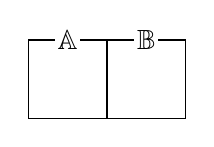
\begin{tikzpicture}
          
            %四角形
            \draw (0,0) rectangle (1,1);
            \draw (1,0) rectangle (2,1);
  
            %ラベル
            \node[set label, text=black] () at (0.5, 1) {$\ds \mathbb{A}$};
            \node[set label, text=black] () at (1.5, 1) {$\ds \mathbb{B}$};
  
          \end{tikzpicture}
        \end{equation*}

        \begin{equation*}
          \begin{split}
            $\ds n(\mathbb{U}) $ & $\ds = n(\mathbb{A}) + n(\mathbb{B}) - n(\mathbb{A \cap B})$\\
            & $\ds = n(\mathbb{A}) + n(\mathbb{B}) \quad (\because \eqref{eq:not-happening-at-the-same-time})$
          \end{split}
        \end{equation*}

        である。\par
        つまりまとめれば

        \begin{breakbox}
          \begin{equation*}
            \begin{split}
              &事象$\ds A, B$が同時に起こらない\\
              &\begin{split}
                \Longrightarrow $\ds A$または & $\ds B$のどちらかが起こる場合の数\\
                & $\ds = A$の起こり方 $\ds + B$の起こり方\\
              \end{split}\\
            \end{split}
          \end{equation*}
        \end{breakbox}

        であり、これを和の法則という。

        \subsubsection{和の法則の成立する例}
          \begin{breakbox}
            大小$\ds 2$個のさいころを投げる。このとき、出る目の和が$\ds 5$の倍数になる場合は何通りあるか求めよ。
          \end{breakbox}

          さいころは$\ds 1$つにつき目の数が$\ds 6$個しかないので書き出せば求められるが、ここでは集合論的に議論しよう。\par
          まず、さいころの目の集合$\ds D$は

          \begin{equation*}
            \begin{split}
              $\ds D \ldef \{ e \in \mathbb{N} \mid 1 \leq e \leq 6 \}$
            \end{split}
          \end{equation*}

          であるので

          \begin{equation*}
            \begin{split}
              $\ds \max D = 6$
            \end{split}
          \end{equation*}

          である。ゆえに$\ds 2$つのさいころの目の和の最大値は

          \begin{equation*}
            \begin{split}
              $\ds \max D + \max D$ & $\ds = 6 + 6$\\
              & $\ds = 12$
            \end{split}
          \end{equation*}

          であるから、考えうる目の和の$\ds 5$の倍数を要素に持つ集合$\ds F$は次のように定義される。

          \begin{equation*}
            \begin{split}
              $\ds F$ & $\ds \ldef \{ f \in \mathbb{N} \mid \exists_{n \in \mathbb{N}} [ f = 5n ] \wedge f \leq (\max D + \max D) \}$\\
              & $\ds = \{ f \in \mathbb{N} \mid \exists_{n \in \mathbb{N}} [ f = 5n ] \wedge f \leq 12 \}$\\
              & $\ds = \{ 5, 10 \}$\\
            \end{split}
          \end{equation*}

          ここで、和が$\ds 5$になるような各さいころの目の組を要素に持つ集合を$\ds A$、和が$\ds 10$になるような組の集合を$\ds B$とすると

          \begin{equation*}
            \begin{split}
              $\ds A$ & $\ds = \{ (1, 4), (2, 3), (3, 2), (4, 1) \}$\\
              $\ds B$ & $\ds = \{ (4, 6), (6, 4), (5, 5) \}$\\
              & $\ds \therefore n(A) = 4, n(B) = 3$
            \end{split}
          \end{equation*}

          となる。\par
          ここに$\ds A$と$\ds B$は同時に起こりえないので、和の法則より

          \begin{equation*}
            \begin{split}
              $\ds n(A \cup B)$ & $\ds = n(A) + n(B)$\\
              & $\ds = 4 + 3$\\
              & $\ds = 7$
            \end{split}
          \end{equation*}

          よって求める場合の数は$\ds 7$通りである。
      
      \subsection{積の法則}
        次に事象$\ds A, B$が同時に起こる状況について議論しよう。
        事象$\ds A, B$に対応する集合は先ほど同様$\ds \mathbb{A}, \mathbb{B}$とし、全事象$\ds U$の集合を$\ds \mathbb{U}$とする。
        つまり$\ds \mathbb{A} \cap \mathbb{B} \ne \varnothing$の状況を考える。\par
        先ほどの$\ds A, B$が同時に起こらない状況では$\ds \mathbb{A} \cap \mathbb{B} = \varnothing$であったために事象$\ds A$を定める情報があれば事象$\ds B$の情報は含まずとも
        $\ds n(\mathbb{U})$を定めることができた。
        しかし同時に起こってしまう場合両者を定める情報がなくてはならない。\par
        具体的には$\ds \mathbb{A} \cap \mathbb{B \ne \varnothing}$ゆえ、事象$\ds A$が起こるからと言って事象$\ds B$が起こらないとは限らないということである。\par

        \begin{equation*}
          \centering
          \begin{tikzpicture}[auto]
        
            \def \circleRadius{1}
            \def \leftCirclePoint{(0, 0)}
            \def \rightCirclePoint{(1, 0)}
            \def \leftCircleNamePoint{(0, 1)}
            \def \rightCircleNamePoint{(1, 1)}
  
            \fill[black!50!white] \leftCirclePoint circle (\circleRadius);
            \scope
              \clip \rightCirclePoint circle (\circleRadius);
              \fill [white] \leftCirclePoint circle (\circleRadius);
            \endscope
            \scope
              \clip \rightCirclePoint circle (\circleRadius);
              \fill [pattern=north west lines] \leftCirclePoint circle (\circleRadius);
            \endscope
            \draw \leftCirclePoint circle (\circleRadius);
            \draw \rightCirclePoint circle (\circleRadius);
  
            \node[set label, text=black] (A) at \leftCircleNamePoint {$\ds \mathbb{A}$};
            \node[set label, text=black] (B) at \rightCircleNamePoint {$\ds \mathbb{B}$};

            \fill[black!50!white] (2.6, 0.3) rectangle (3, 0.7);
            \node[set label, text=black] (_A) at (4.2, 0.5) {事象$\ds A$が起こる};

            \fill[pattern=north west lines] (2.6, -0.3) rectangle (3, -0.7);
            \node[set label, text=black] (_B) at (4.55, -0.5) {事象$\ds A$も$\ds B$も起こる};
  
          \end{tikzpicture}
        \end{equation*}

        ここで議論が行き詰ってしまった原因は、事象$\ds A, B$に対する全事象の集合$\ds \mathbb{U}$の定義の仕方が悪かったことにある。
        つまり、試行によって$\ds A$または$\ds B$の根元事象、つまり要素が$\ds 1$つ決まることに対応するように$\ds \mathbb{U}$を定義していなかったということである。\par
        そこでこの定義を改善してみよう。\par
        先ほどまでの定義では$\ds A$または$\ds B$の根元事象\overdot{1}\overdot{つ}\overdot{1}\overdot{つ}に対応させていなかったので、次のように$\ds U$の集合$\ds \mathbb{U'}$を再定義する。

        \begin{breakbox}
          $\ds a \in \mathbb{A}, b \in \mathbb{B}$とするとき$\ds (a, b) \in \mathbb{U'}$となるように定義する。\par
          つまり
          \begin{equation*}
            \begin{split}
              $\ds \mathbb{U'} \ldef \{ (a, b) \mid a \in \mathbb{A}, b \in \mathbb{B} \}$
            \end{split}
          \end{equation*}
        \end{breakbox}

        また、事象$\ds A, B$に対応する集合をこの$\ds \mathbb{U'}$を用いて表すと

        \begin{equation*}
          \begin{split}
            $\ds \mathbb{A'}$ & $\ds \ldef \{ (a, b) \mid (a, b) \in \mathbb{U'} \wedge a \ne \varnothing \}$\\
            $\ds \mathbb{B'}$ & $\ds \ldef \{ (a, b) \mid (a, b) \in \mathbb{U'} \wedge b \ne \varnothing \}$\\
            $\ds \therefore$ & $\ds \mathbb{A'} \subset \mathbb{U'}, \mathbb{B'} \subset \mathbb{U'}$
          \end{split}
        \end{equation*}

        となる。\par
        ちなみに、事象が$\ds A$ではないとき$\ds a = \varnothing$、$\ds B$ではないとき$\ds b = \varnothing$であり、
        それゆえどちらでもないとき$\ds (a, b) = (\varnothing, \varnothing)$と対応する。

        ここで、事象$\ds A, B$が同時に起こる状況において、特に
        
        \begin{eqnarray}
          \begin{split}
            「事象$\ds A$のすべての場合で事象$\ds B$が一律$\ds b$通り起こるとき」\label{term:ab}
          \end{split}
        \end{eqnarray}
        
        を考えてみよう。\par
        事象$\ds B$のうち$\ds b$通りを$\ds \mathbb{B'}$の部分集合$\ds \mathbb{C}$として表すと、この条件\eqref{term:ab}の下では$\ds \mathbb{A'}$は

        \begin{eqnarray}
          \begin{split}
            $\ds \mathbb{A'} = \{ (a, b) \mid a \in \mathbb{A} \wedge a \ne \varnothing, b \in \mathbb{C} \wedge b \ne \varnothing \}$ \label{eq:equaltion-of-A'1}
          \end{split}
        \end{eqnarray}

        と表される。これは集合の直積で表現すれば

        \begin{eqnarray}
          \begin{split}
            $\ds \mathbb{A'} = \mathbb{A} \times \mathbb{C}$ \label{eq:equaltion-of-A'2}
          \end{split}
        \end{eqnarray}

        \begin{equation*}
          \centering
          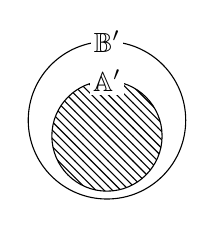
\begin{tikzpicture}
          
            \def \circleARadius{0.7}
            \def \circleBRadius{1}
            \def \circleAPoint{(4, -0.2)}
            \def \circleBPoint{(4, 0)}
            \def \circleANamePoint{(4, \circleARadius-0.2)}
            \def \circleBNamePoint{(4, \circleBRadius)}

            \fill[pattern=north west lines] \circleAPoint circle (\circleARadius);
            \draw                           \circleAPoint circle (\circleARadius);
            \draw                           \circleBPoint circle (\circleBRadius);
            \node[set label, text=black] (A') at \circleANamePoint {$\ds \mathbb{A'}$};
            \node[set label, text=black] (B') at \circleBNamePoint {$\ds \mathbb{B'}$};
  
          \end{tikzpicture}
        \end{equation*}

        \begin{eqnarray}
          \begin{split}
            & $\ds \therefore \mathbb{A'}\subset \mathbb{B'}$\\
            & $\ds \therefore \mathbb{A'} \cap \mathbb{B'} = \mathbb{A'}$ \label{eq:A'-cap-B'}\\
          \end{split}
        \end{eqnarray}

        よって「事象$\ds A$と$\ds B$が同時に起こる場合の数」は\eqref{eq:equaltion-of-A'1}と\eqref{eq:A'-cap-B'}より

        \begin{equation*}
          \begin{split}
            $\ds n(\mathbb{A'} \cap \mathbb{B'})$ & $\ds = n(\mathbb{A'})$\\
            & $\ds = n(\mathbb{A} \times \mathbb{C})$ \quad (\because \eqref{eq:equaltion-of-A'2})\\
            & $\ds = n(\mathbb{A}) \times n(\mathbb{C})$\\
            & \left(\because\begin{split}
              & 事象$\ds A, B$は有限通りゆえ\\
              & \quad \quad \quad 有限集合直積の濃度\\
            \end{split}\right)\\
            & $\ds = a \times b$
          \end{split}
        \end{equation*}

    \end{multicols*}

\end{document}
